\documentclass[a4paper,12pt]{article}

\usepackage{ngerman}
\usepackage[utf8]{inputenc}
\usepackage{amsmath}
\usepackage{amssymb}
\usepackage{multicol}
\usepackage{framed}
\usepackage{graphicx}
\usepackage{hyperref}

\usepackage[left=2.2 cm,right=2.2 cm,top=1.5cm,bottom=2.0cm]{geometry}

\newcounter{aufgnr}

\begin{document}
\begin{center}
\section*{Die Von-Neumann-Architektur}
\subsection*{Beschreibung des Modellrechners KUR2}
\end{center}

\hrule
\vspace{.5cm}

Der klassische Universalrechner 2 oder KUR2 ist ein konkretes Rechnermodell nach den Von-Neumann'schen Vorgaben.\\

\subsection*{\underline{Das Rechenwerk}}
\begin{figure}[h]
\centering
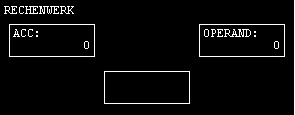
\includegraphics[scale=.75]{ALU.png}
\end{figure}

Das Rechenwerk führt alle Rechenoperationen aus. Außerdem dient es als Zwischenspeicher für Daten, die eingegeben, ausgegeben oder verschoben werden sollen. Es hat zwei interne Speicherzellen:
\begin{itemize}
\item \underline{ACC:} Der Accumulator ACC speichert alle Ergebnisse von Rechnungen und stelle die Quelle für alle ausgehenden Datenverbindungen dar. Außerdem ist er bei Rechenoperationen der erste Operand (wichtig z.B. bei der Subtraktion und der Division)
\item \underline{OPERAND:} In dieser Speicherzelle werden eingehende Daten zwischengespeichert und bei Rechenoperationen als zweiter Operand genutzt
\end{itemize}


\subsection*{\underline{Das Steuerwerk}}
\begin{figure}[h]
\centering
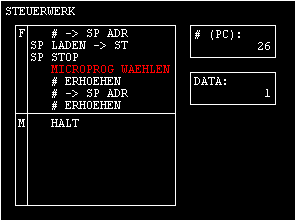
\includegraphics[scale=.75]{ControlUnit.png}
\end{figure}

Das Steuerwerk stellt die zentrale Steuerung der Maschine dar. Von hier aus werden Steuerbefehle an die anderen Komponenten gegeben. Welche Steuerbefehle gegeben werden hängt von der aktuell ausgeführten Programmzeile ab. Diese wird zunächst in der \underline{Befehlholphase} aus dem Speicher geladen und anschließend in der \underline{Befehlsausführungsphase} ausgeführt. Letzteres bedeutet, dass eine Folge von Steuerbefehlen an die anderen Komponenten gegeben wird. Diese Folge wird als \underline{Microprogramm} bezeichnet.\\
\newpage
Das Steuerwerk besitzt zwei interne Speicherzellen:
\begin{itemize}
\item \underline{\# (PC):} Der Programmzähler \# (oder PC) speichert die Speicheradresse des nächsten Programmbefehls
\item \underline{DATA:} Die Speicherzelle DATA wird als Zwischenspeicher für alle eingehenden Datenverbindungen genutzt
\end{itemize}
Weiterhin besitzt das Steuerwerk zwei Stellen, an denen Microprogramme gespeichert werden:
\begin{itemize}
\item \underline{F:} Das \underline{Befehlholmicroprogramm} (FETCH) dient dazu, den nächsten Befehl aus dem Speicher ins Steuerwerk zu laden und das zugehörige Microprogramm in M zu auszuwählen
\item \underline{M:} Das \underline{Microprogramm} M enthält die Folge von Steuerbefehlen, die an die anderen Komponenten gesendet wird, um den aktuellen Programmbefehl auszuführen
\end{itemize}


\subsection*{\underline{Das Speicherwerk}}
\begin{figure}[h]
\centering
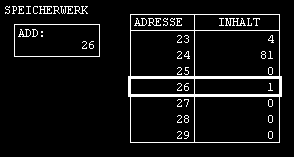
\includegraphics[scale=.75]{MemoryUnit.png}
\end{figure}

Das Speicherwerk verwaltet den Hauptspeicher, welcher das auszuführende Programm und alle anderen Daten enthält. Es ist dafür zuständig, den anderen Komponenten Daten bereit zu stellen und verarbeitete Daten zu speichern. Es hat eine besondere Speicherzelle ADD, die Adresse, auf welche zugegriffen werden soll. Bei Veränderung von ADD wird der Speicher so eingestellt, dass der Wert mit der Speicheradresse ADD ausgegeben oder überschrieben werden kann.


\subsection*{\underline{Das Eingabewerk \& das Ausgabewerk}}
\begin{figure}[h]
\centering
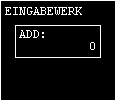
\includegraphics[scale=.75]{InputUnit.png}
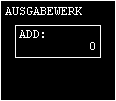
\includegraphics[scale=.75]{OutputUnit.png}
\end{figure}
Das Eingabewerk und das Ausgabewerk stellen Möglichkeiten bereit, um mit der \glqq Außenwelt\grqq~zu interagieren. Sie erlauben der Maschine, Eingaben von Eingabegeräten entgegen zu nehmen und Ausgaben an Ausgabegeräte zu senden. Sie besitzen jeweils eine interne Speicherzelle ADD, welche dazu genutzt wird, um festzulegen, welches Ein- bzw. Ausgabegerät angesprochen werden soll.


\end{document}